%%%%%%%%%%%%%%%%%%%%%%%%%%%%%%%%%%%%%%%%%
% Beamer Presentation
% LaTeX Template
% Version 1.0 (10/11/12)
%
% This template has been downloaded from:
% http://www.LaTeXTemplates.com
%
% License:
% CC BY-NC-SA 3.0 (http://creativecommons.org/licenses/by-nc-sa/3.0/)
%
%%%%%%%%%%%%%%%%%%%%%%%%%%%%%%%%%%%%%%%%%

%----------------------------------------------------------------------------------------
%	PACKAGES AND THEMES
%----------------------------------------------------------------------------------------

\documentclass{beamer}

\mode<presentation> {

% The Beamer class comes with a number of default slide themes
% which change the colors and layouts of slides. Below this is a list
% of all the themes, uncomment each in turn to see what they look like.

%\usetheme{default}
%\usetheme{AnnArbor}
%\usetheme{Antibes}
%\usetheme{Bergen}
%\usetheme{Berkeley}
%\usetheme{Berlin}
%\usetheme{Boadilla}
%\usetheme{CambridgeUS}
%\usetheme{Copenhagen}
%\usetheme{Darmstadt}
%\usetheme{Dresden}

%\usetheme{Frankfurt}

%\usetheme{Goettingen}
%\usetheme{Hannover}
%\usetheme{Ilmenau}
%\usetheme{JuanLesPins}
%\usetheme{Luebeck}
%\usetheme{Madrid}
%\usetheme{Malmoe}
%\usetheme{Marburg}
%\usetheme{Montpellier}
%\usetheme{PaloAlto}
%\usetheme{Pittsburgh}

%\usetheme{Rochester}
\usetheme{Singapore}

%\usetheme{Szeged}
%\usetheme{Warsaw}

% As well as themes, the Beamer class has a number of color themes
% for any slide theme. Uncomment each of these in turn to see how it
% changes the colors of your current slide theme.

%\usecolortheme{albatross}
%\usecolortheme{beaver}
%\usecolortheme{beetle}
%\usecolortheme{crane}
%\usecolortheme{dolphin}
%\usecolortheme{dove}
%\usecolortheme{fly}
%\usecolortheme{lily}
%\usecolortheme{orchid}
%\usecolortheme{rose}
%\usecolortheme{seagull}
%\usecolortheme{seahorse}
%\usecolortheme{whale}
%\usecolortheme{wolverine}

%\setbeamertemplate{footline} % To remove the footer line in all slides uncomment this line
%\setbeamertemplate{footline}[page number] % To replace the footer line in all slides with a simple slide count uncomment this line

%\setbeamertemplate{navigation symbols}{} % To remove the navigation symbols from the bottom of all slides uncomment this line
}

\usepackage{graphicx} % Allows including images
\usepackage{booktabs} % Allows the use of \toprule, \midrule and \bottomrule in tables
\usepackage{array}
\usepackage{color}
\usepackage{url}
\usepackage[T2A]{fontenc}
\usepackage[utf8]{inputenc}
\usepackage[export]{adjustbox}
\usepackage{amsmath}
\usepackage{sidecap}
\usepackage{listings}
\usepackage{mathtools}
\usepackage[normalem]{ulem}
%\usepackage[english,serbian]{babel}
\usepackage[english,serbianc]{babel} %ukljuciti babel sa ovim opcijama, umesto gornjim, ukoliko se koristi cirilica

\lstset{breakatwhitespace,
language=C++,
columns=fullflexible,
keepspaces,
breaklines,
tabsize=4,
showstringspaces=false,
basicstyle=\ttfamily,
extendedchars=true}

%----------------------------------------------------------------------------------------
%	TITLE PAGE
%----------------------------------------------------------------------------------------

\title[Семинарски МСНР]{Примена техника машинског учења у статичкој верификацији софтвера}
\author{	Лазар Ранковић 1099/2016 \\
		Немања Мићовић 1085/2016 \\
		Урош Стегић 447/2016
}
\institute[МАТФ]{Математички факултет}
\date{\today}

\begin{document}

\begin{frame}
\titlepage
\end{frame}

\begin{frame}
\frametitle{Садржај}
\tableofcontents
\end{frame}

%----------------------------------------------------------------------------------------
%	PREZENTACIJA
%----------------------------------------------------------------------------------------

%-----------------------------------------------------------------
\section{Статичка верификација}

\begin{frame}
\frametitle{Мотивација}
\begin{itemize}
    \item Важност процеса верификације софтвера
    %\item Не производе се више јафолитанке :()
%-----------------------------------------------------------------
\end{itemize}
\end{frame}
\begin{frame}
\frametitle{Увод}
\begin{itemize}
	\item Верификација?
 	\item Основни приступи
    \begin{itemize}
    \item Динамичка верификација
    \item Статичка верификација
    \end{itemize}
 	\item Халтинг проблем \emph{(енгл. halting problem)}
\end{itemize}
\end{frame}
%-----------------------------------------------------------------
\begin{frame}
\frametitle{Методи статичке верификације}
\begin{itemize}
	\item Апстрактна интерпретација
 	\item Проверавање модела
 	\item Симболичко израчунавање
\end{itemize}
\end{frame}
%-----------------------------------------------------------------

%-----------------------------------------------------------------
\section{Машинско учење}

\begin{frame}
\frametitle{Машинско учење}
\framesubtitle{Увод}
\begin{itemize}
 	\item Грађење и употреба алгоритама који генерализују
	\item Писање програма који се прилагођавају
	\item Статистичко учење из података
\end{itemize}
\end{frame}
%-----------------------------------------------------------------
\begin{frame}
\frametitle{Машинско учење}
\framesubtitle{Мотивација}
\begin{itemize}
 	\item Алгоритамски \sout{нерешиви} тешко решиви проблеми
 	\item Задаци које човек лако решава
	\item Предиктивна анализа
\end{itemize}
\end{frame}
%-----------------------------------------------------------------
\begin{frame}
\frametitle{Машинско учење}
\framesubtitle{Класификација}
\begin{itemize}
 	\item Препознавање објеката на фотографији
 	\item Разврставање непожељне поште
 	\item Класификација стања програма
\end{itemize}
\end{frame}
%-----------------------------------------------------------------
\begin{frame}
\frametitle{Машинско учење}
\framesubtitle{Стабло одлучивања}
\begin{figure}
\centering
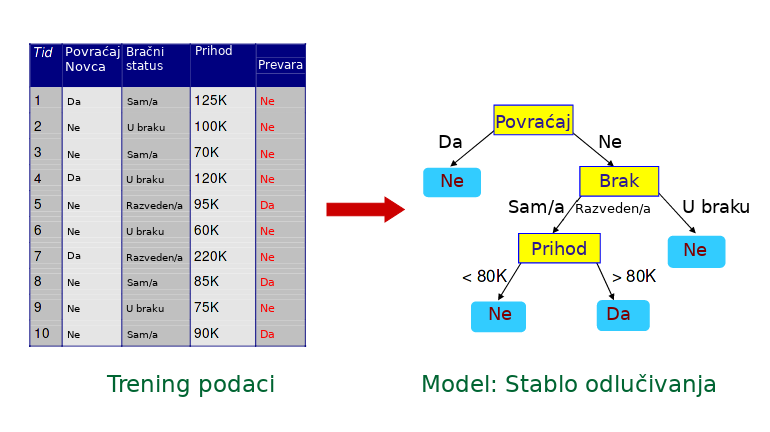
\includegraphics[scale=0.4]{slike/decision_tree.png}
\end{figure}
\end{frame}
%-----------------------------------------------------------------
\begin{frame}
\frametitle{Машинско учење}
\framesubtitle{Метода потпорних вектора}
\begin{figure}
\centering
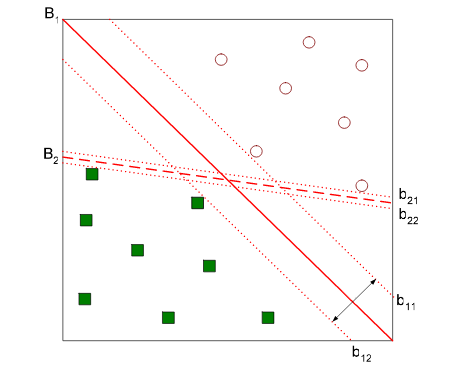
\includegraphics[scale=0.4]{slike/svm.png}
\end{figure}
\end{frame}
%-----------------------------------------------------------------
\begin{frame}
\frametitle{Машинско учење}
\framesubtitle{Још мало мотивације}
\begin{itemize}
 	\item Магија у НП проблемима
 	\item Машинско учење на белом коњу
\end{itemize}
\end{frame}
%-----------------------------------------------------------------

\section{Примене МУ у статичкој верификацији}
\begin{frame}[fragile]
\frametitle{Проналажење интерполанти - потпорни вектори}

\begin{itemize}
    \item Делимо скуп стања програма на скупове $A$ и  $B$
    \item $A$ и $B$ се описују формулом логике првог реда
    \item $A$ садржи вредности $x$ и  $y$ након линија 1, 2, 3
    \item $B$ садржи вредности $x$ и $y$ након линија 4, 5, 6 и 7
\end{itemize}
\begin{columns}
\begin{column}{0.3\textwidth}
    \begin{center}
        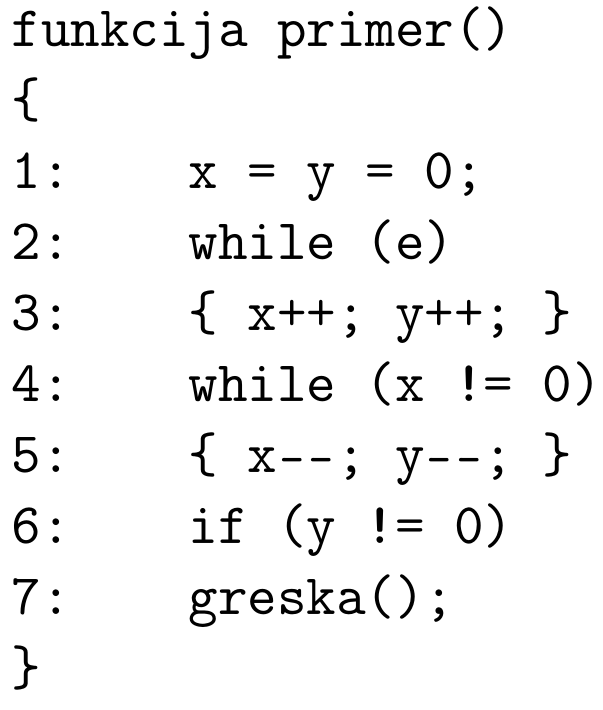
\includegraphics[scale=0.17]{./slike/interpolant_code2.png}
    \end{center}
\end{column}
\begin{column}{0.7\textwidth}  %%<--- here
	\begin{itemize}
    \item Интерполанта је доказ да су скупови $A$ и  $B$ дисјунктни
    \item Доказивач теорема рачуна вредности за променљиве $x$ и  $y$
    \item Добија се скуп инстанци над којима се може тренирати модел машинског учења
    \end{itemize}
\end{column}
\end{columns}

\end{frame}
%-----------------------------------------------------------------
%\begin{frame}
%\frametitle{Проналажење интерполанти - потпорни вектори}
%\begin{itemize}
    %\item Делимо скуп стања програма на скупове $A$ и  $B$
    %\item $A$ и $B$ се описују формулом логике првог реда
    %\item $A$ садржи вредности $x$ и  $y$ након линија 1, 2, 3
    %\item $B$ садржи вредности $x$ и $y$ након линија 4, 5, 6 и 7
    %\item Интерполанта је доказ да су скупови $A$ и  $B$ дисјунктни
    %\item Доказивач теорема рачуна вредности за променљиве $x$ и  $y$
    %\item Добија се скуп инстанци над којима се може тренирати модел машинског учења
%\end{itemize}
%\end{frame}
%-----------------------------------------------------------------
\begin{frame}
\frametitle{Проналажење интерполанти - потпорни вектори}
\begin{columns}
\begin{column}{0.5\textwidth}
	\begin{itemize}
		\item Модел добијен применом метода потпорних вектора
		\item Приказане праве одговарају једначинама:
		$ p1: 2y = 2x + 1 $
		$ p2: 2y = 2x - 1 $
		\item Можемо извести интерполанту $ 2y \leq 2x + 1 \land 2y \geq 2x - 1 $
        \item Инваријанта $x=y$ се може добити транслирањем правих што ближе позитивним инстанцама
	\end{itemize}
\end{column}
\begin{column}{0.5\textwidth}  %%<--- here
	\begin{center}
		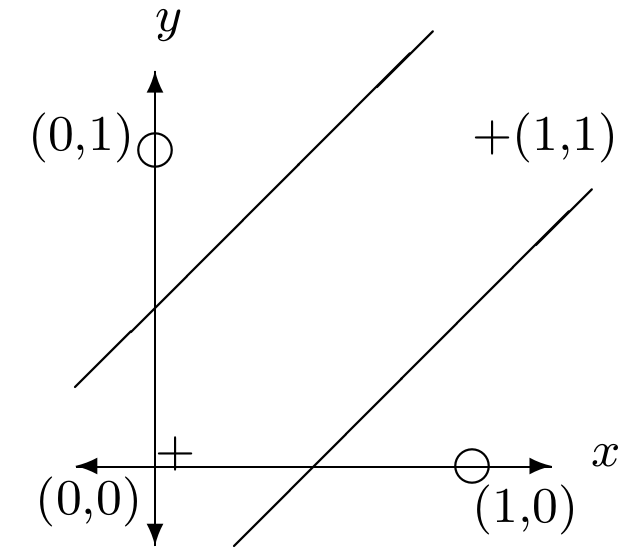
\includegraphics[scale=0.22]{./slike/interpolant.png}
	\end{center}
\end{column}
\end{columns}
\end{frame}
%-----------------------------------------------------------------
\begin{frame}
\frametitle{Грађење класификатора нетачне инваријанте}
\begin{itemize}
    \item Рангирају се својста програма по вероватноћи за стварање грешке
    \item Циљ је програмеру понудити листу својстава које потенцијално треба проверити
        %\begin{center}
        %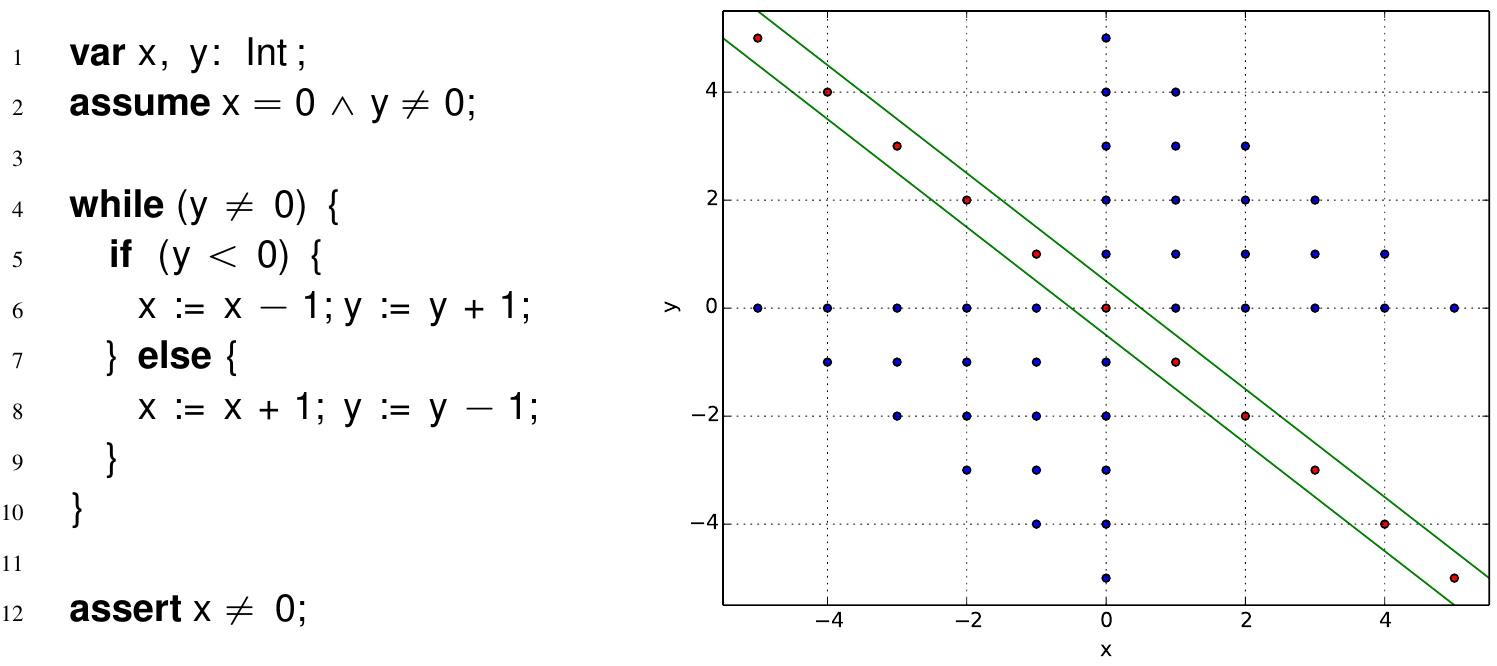
\includegraphics[scale=0.19]{./slike/interpolant2.png}    
    %\end{center}
\end{itemize}

\begin{columns}
\begin{column}{0.55\textwidth}
    \begin{center}
		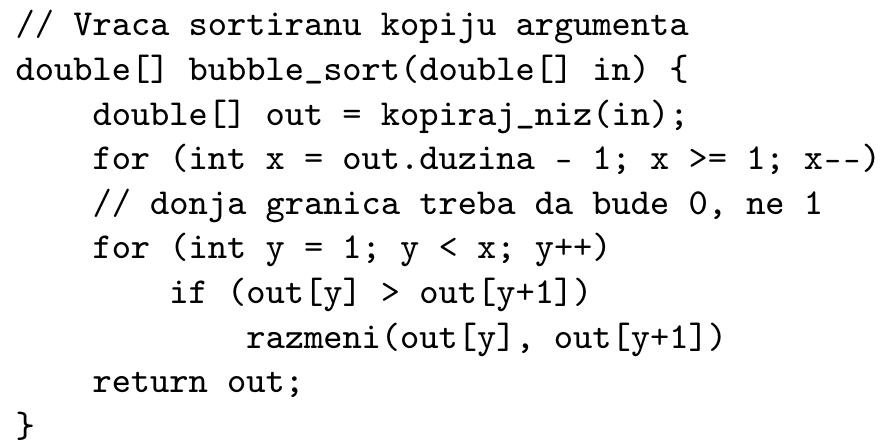
\includegraphics[scale=0.15]{./slike/latent_code2.png}
    \end{center}
\end{column}
\begin{column}{0.45\textwidth}  %%<--- here
	\begin{center}
		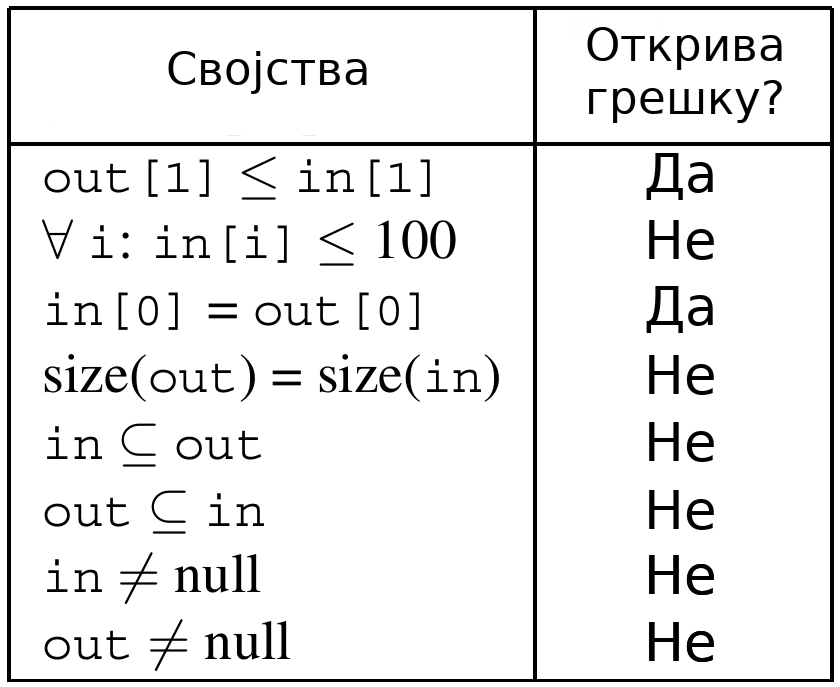
\includegraphics[scale=0.13]{./slike/latent_examples.png}
	\end{center}
\end{column}
\end{columns}


\end{frame}
%-----------------------------------------------------------------
\begin{frame}[fragile]
\frametitle{Грађење класификатора нетачне инваријанте}
\begin{itemize}
\item Користи се \textsc{Daikon} динамички детектор инваријанти који може да проверава:
    \begin{itemize}
        \item уређење ($x \leq y$)
        \item опсег ($a \leq x \leq b$)
        \item линеарне везе ($z = ax + by + c$)
        \item и друге
    \end{itemize}
\item Добијена својства се кодирају у векторе и примењује се метода машинског учења
\end{itemize}

%\begin{center}
    %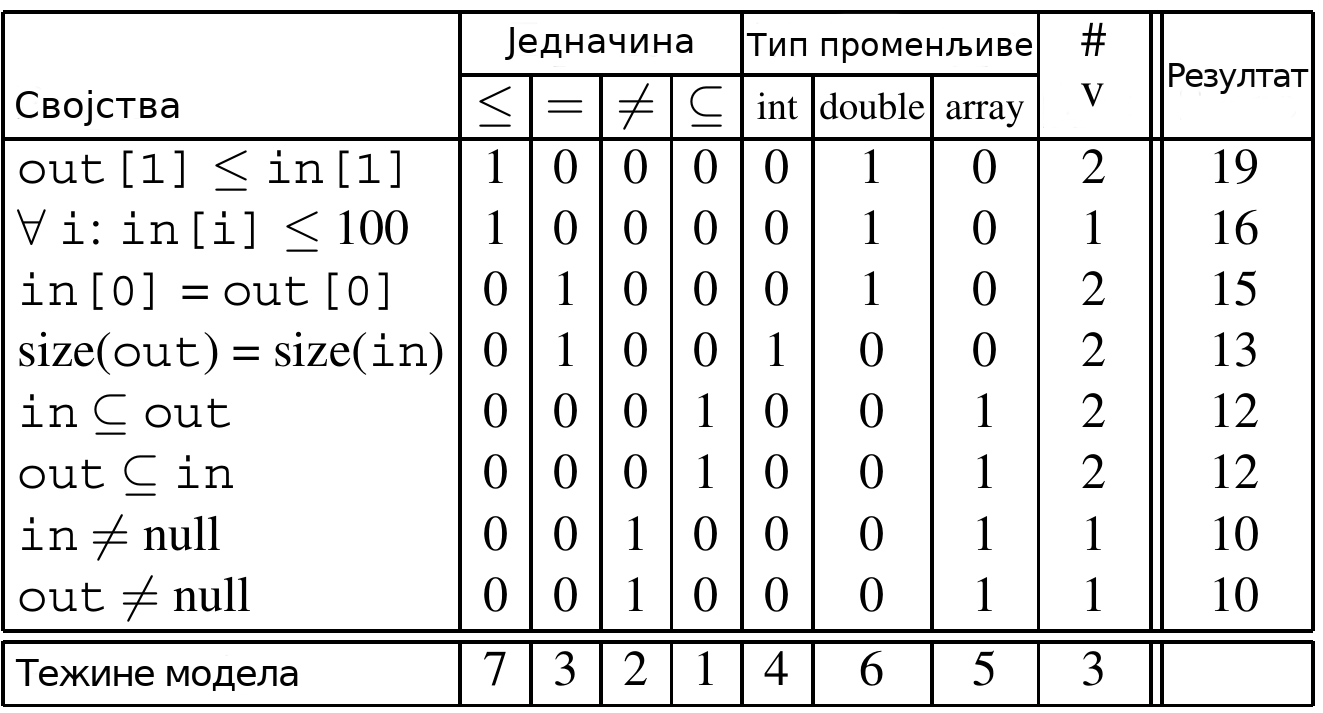
\includegraphics[scale=0.15]{./slike/latent_errors_table.png}
%\end{center}

\begin{columns}
\begin{column}{0.35\textwidth}
    \begin{center}
        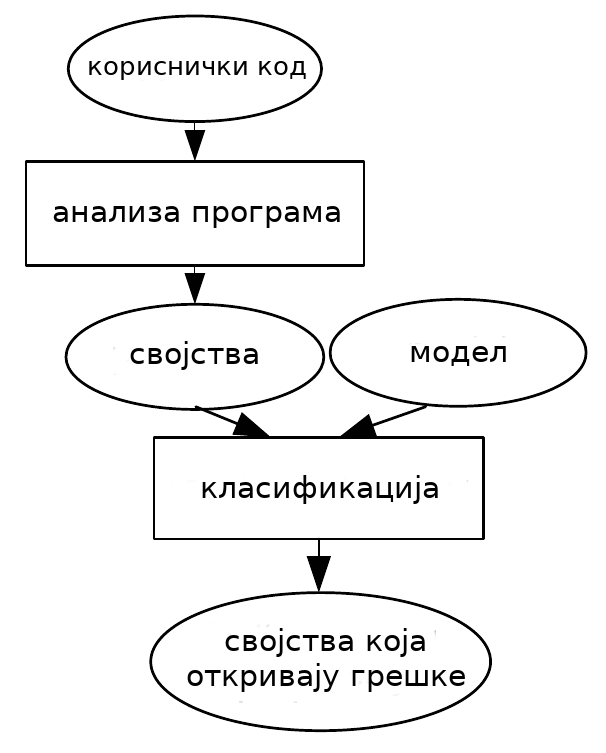
\includegraphics[scale=0.16]{./slike/latent_flow.png}
    \end{center}
\end{column}
\begin{column}{0.65\textwidth}  %%<--- here
    \begin{center}
        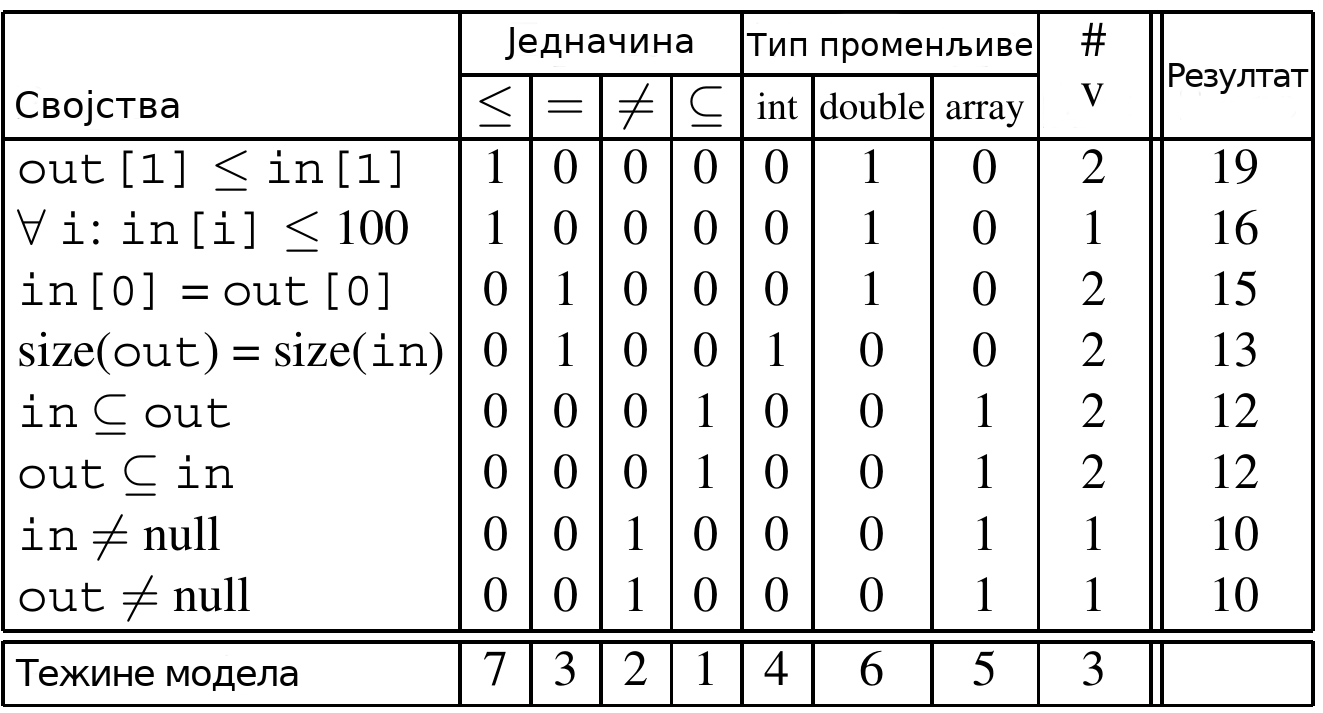
\includegraphics[scale=0.14]{./slike/latent_errors_table.png}
    \end{center}
\end{column}
\end{columns}
\end{frame}
%-----------------------------------------------------------------
\begin{frame}
\frametitle{Закључак}
\begin{itemize}
    \item Машинско учење итекако може имати примену у верификацији софтвера
    \item Добијени резултати су упоредиви а негде и бољи од традиционалних метода
\end{itemize}
\end{frame}
%-----------------------------------------------------------------
\begin{frame}
\Huge{\centerline{Хвала на пажњи}}
\end{frame}
%-----------------------------------------------------------------



%-----------------------------------------------------------------
\end{document}
